\subsection{inciso 1.a}

Se midieron las salidas de una entrada cuadrada $D = 0,5$. Se obtuvieron los siguientes resultados:

\begin{figure}[htbp]
    \centering
    % Primera fila: 3 imágenes
        \begin{subfigure}[b]{0.31\textwidth}
        \centering
        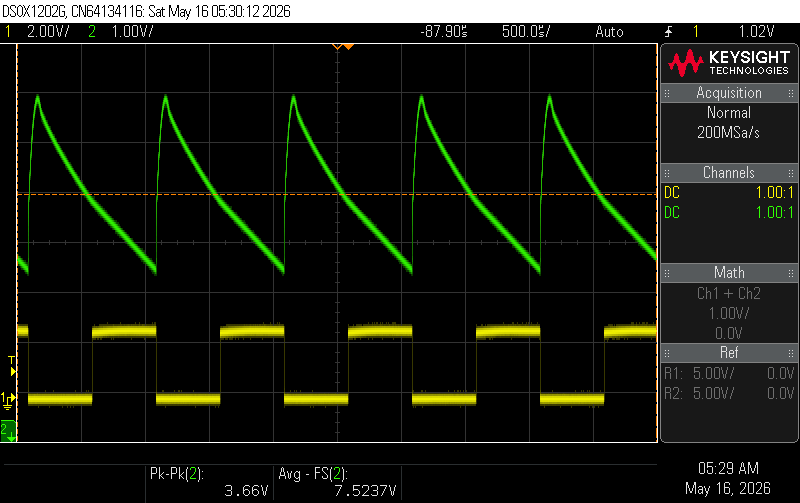
\includegraphics[width=\textwidth]{imagenes/tp3_a1k.png}
        \caption{Ripple y $V_{medio}$ medido a $f = 1kH$.}
         \label{fig:a_1}
    \end{subfigure}
    \hfill
    \begin{subfigure}[b]{0.31\textwidth}
        \centering
        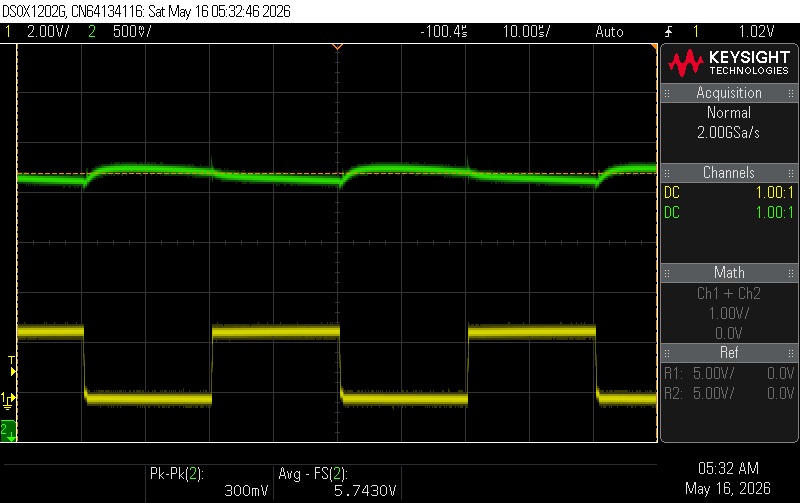
\includegraphics[width=\textwidth]{imagenes/tp3_a25k.png}
        \caption{Ripple y $V_{medio}$ medido a $f = 25kH$. En ltspice $V_{medio} = 6,05V$}
        \label{fig:a_25}
    \end{subfigure}
    \hfill
    \begin{subfigure}[b]{0.31\textwidth}
        \centering
        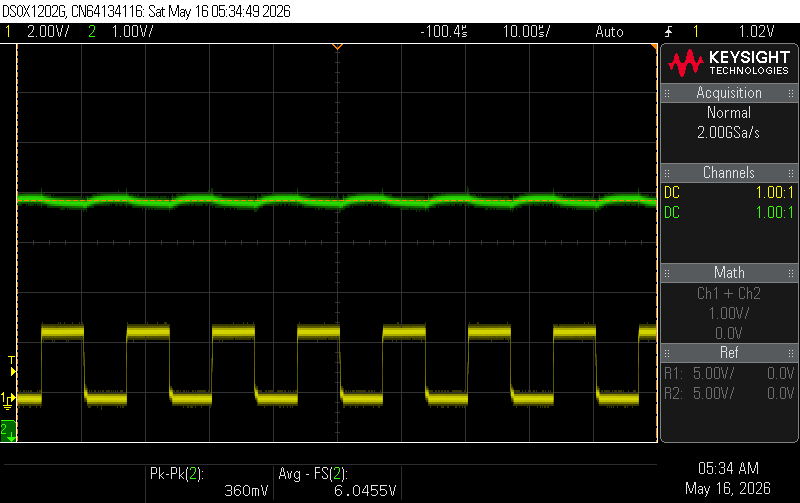
\includegraphics[width=\textwidth]{imagenes/tp3_a75k.png}
        \caption{Ripple y $V_{medio}$ medido a $f = 75kH$. En ltspice $V_{medio} = 6,69V$}
         \label{fig:a_75}
    \end{subfigure}

    \vspace{2mm} % Espacio vertical comprimido entre filas

    % Segunda fila: La imagen restante (y puedes agregar más aquí)
    \begin{subfigure}[b]{0.31\textwidth}
        \centering
        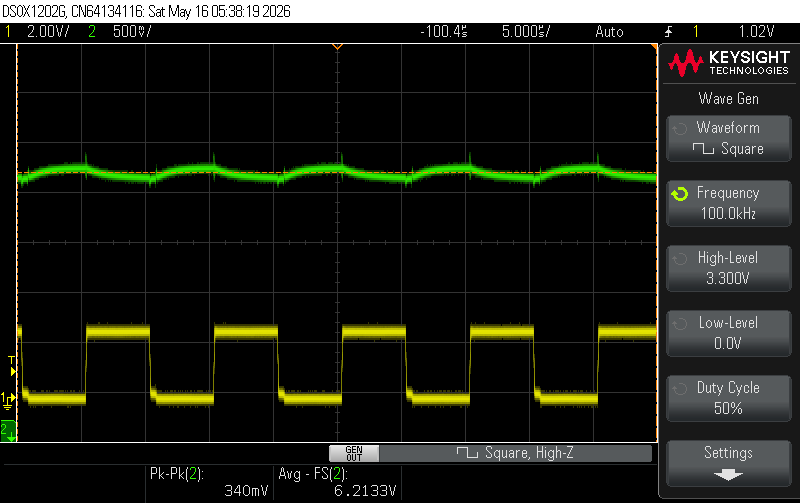
\includegraphics[width=\textwidth]{imagenes/tp3_a100k.png}
        \caption{Ripple y $V_{medio}$ medido a $f = 100kH$. En ltspice $V_{medio} = 7,05V$}
         \label{fig:a_100}
    \end{subfigure}
        \begin{subfigure}[b]{0.31\textwidth}
        \centering
        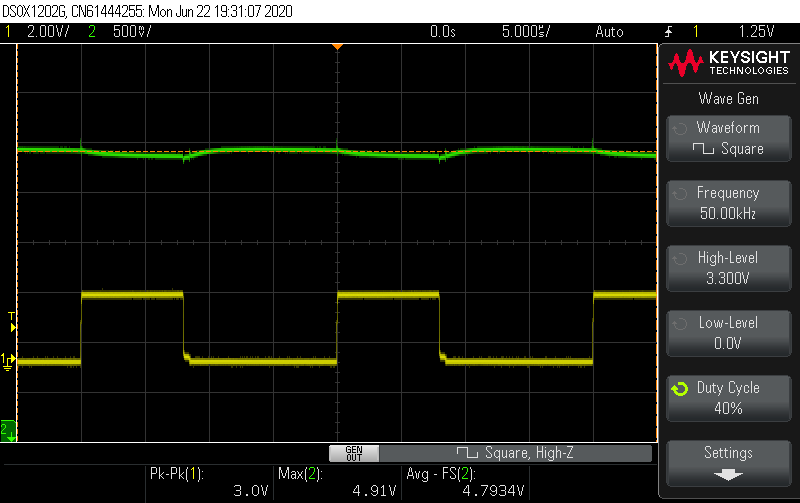
\includegraphics[width=\textwidth]{imagenes/tp3_b_d40.png}
        \caption{Duty cicle 40}
         \label{fig:b_D40}
    \end{subfigure}
        \begin{subfigure}[b]{0.31\textwidth}
        \centering
        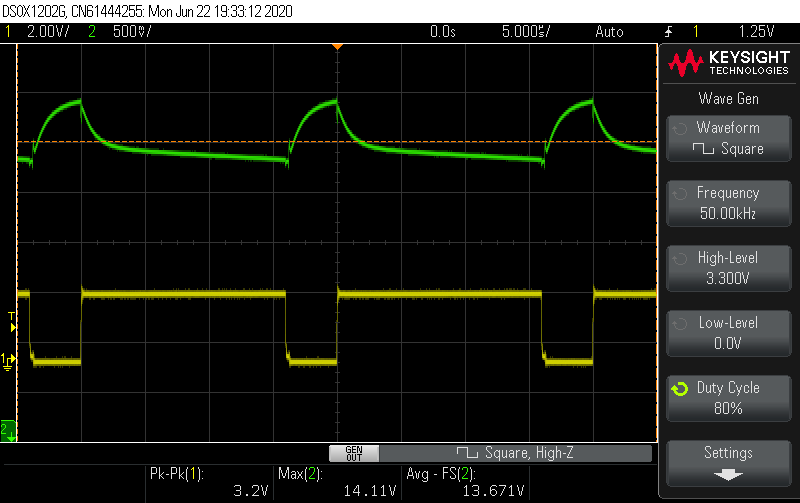
\includegraphics[width=\textwidth]{imagenes/tp3_b_d80.png}
        \caption{Duty cicle 80}
         \label{fig:b_D80}
    \end{subfigure}
    % Si quisieras llenar la fila, añadirías dos subfigures más aquí siguiendo el mismo patrón
    \caption{Señal amarilla entrada y señal verde la salida}
\end{figure}

Se midieron los valores de 25k a 100k. Observando las figuras \ref{fig:a_25}, \ref{fig:a_75} y \ref{fig:a_100}, se observó que la salida del sistema, mantuvo el nivel de ripple estable, mientras que la tensión media de salida del mismo iba en aumento. No obstante, al medir una frecuencia de 1kH, figura \ref{fig:a_1}, se observó una diferencia en el nivel de ripple de salida. Esto se explica ya que al reducir el tiempo de carga del capacitor, este posee menos energía para mantener la tensión, aumentando el ripple. \par
Otra diferencia observada, fue que a una $f = 1kH$ no se cumplió la tendencia del valor medio de tensión de salida. En este caso se observó una salida mucho mayor, a las vistas a altas frecuencias. Esto se puede explicar debido a que al tener mayor tiempo de carga, el núcleo se puede saturar bridando mayores corrientes de salida.\par

Finalmente contrastando estos resultados con los simulados en el LTspice se observó una diferencia en la tensión media de la salida. Se observó que la salida en LTsipce es mayor a la vista en el osciloscopio. Esto se atribuye a que la simulación no considera algunos efectos no menores como las perdidas en el núcleo del inductor.

\subsection{b}

Se estudió la respuesta del circuito al modificar el duty cycle de la salida. En un convertidor Boost la salida del circuito cumple $V_{out} = \frac{V_{in}}{1-D} - V_D$ con $D$ el duty cycle y $V_D = 0,7V$ la caída del diodo. Se hizo un barrido de la respuesta del duty cycle recorriendo de a 0,20. Se observaron los siguientes resultados (observar figuras \ref{fig:b_D40} y          \ref{fig:b_D80}). \par

Se observó que al aumentar el duty cycle, el ripple aumentaba al mismo tiempo que aumentaba la tensión media. Al tratarse de un circuito con una tensión de salida con una componente DC mucho más grande que el ripple, se cumple que $V_{RMS} \approx V_{media}$. Por tal motivo el caso en el que más potencia se disipa es D=0,8 cuando hay mayor $V_{media}$. La potencia disipada fue de $P_{220\Omega}= \frac{V_{media}^2}{R} = 0,85W$.\par

Se mostraron las dos mediciones de $D= 40\%$ y $D=80\%$ para mostrar la diferencia en el ripple. También se puede observar que en el caso de 40\% de duty cycle, la ecuación teórica arroja una tensión de salida de $4,8 V$, muy parecida con la medida. En cambio al aumentar el duty cicle (a partir de 0,7), esta formula se empieza a alejar del valor medido experimentalmente.
